%
% dualraum.tex -- kapitel über den Dualraum
%
% (c) 2017 Prof Dr Andreas Müller, Hochschule Rapperswil
%
\chapter{Dualität}
In der Anfängervorlesung lernt man die Transposition als Operation kennen,
die Zeilen und Spalten einer Matrix vertauscht.
Doch dies ist eine oberflächliche Betrachtungsweise.
In einer strukturelleren Betrachtungsweise macht die Transposition
aus einem Vektor eine Linearform.
Die Transoposition ist daher nur der äusserliche Ausdruck der viel
allgemeineren Konstruktion des Konzepts der Dualität.

Zu jedem Vektorraum $V$ gibt es den Vektorraum $V*$ bestehend aus
allen Linearformen auf $V$.
Für endlichdimensionale Vektorräume $V$ ist auch $V^*$ endlich dimensional.
Wir können sogar zu jeder Basis von $V$ eine passende duale Basis von
$V^*$ finden.
In Matrxdarstellung können wir $V$ mit Spaltenvektoren beschreiben,
die Linearformen sind in diesem Bild die Zeilenvektoren.
Dies wirft ein neues Licht auf die Regel Zeile $\times$ Spalte der
Matrizenrechnung.


%
% linearform.tex -- Abschnitt über Linearformen
%
% (c) 2017 Prof Dr Andreas Müller, Hochschule Rapperswil
%

\section{Linearformen}
\rhead{Linearformen}
Der Begriff der Linearform ist offensichtlich nicht auf endlichdimensionale
Vektorräume beschränkt.
Wir wollen in diesem Abschnitt die Beobachtungen, die wir für Zeilen-
und Spaltenvektoren gemacht haben, auf beliebige Vektoren verallgemeinern.

\subsection{Notation}
Sei $V$ ein $K$-Vektorraum.
Der Vektorraum $\operatorname{Hom}(V,K)$, ebenfalls ein $K$-Vektorraum,
besteht aus linearen Abbildungen von $V$ mach $K$.
Normalerweise schreibt man $l(v)$ für den Wert einer Linearform
$l\in\operatorname{Hom}(V,K)$ auf dem Vektor $v\in V$.
Diese Notation passt aber nicht gut zur Matrizenschreibweise aus
Abschnitt~\ref{section:dualraum:zeilenspalten}.
Wir schreiben daher 
\[
\langle l,v\rangle = l(v),
\]
dies ähnelt viel mehr der Produktnotation für Zeilen- und Spaltenvektoren.

\subsection{Der Dualraum}
Den Vektorraum $\operatorname{Hom}(V,K)$ haben wir
als Spezialfall des Vektorraums $\operatorname{Hom}(V,U)$
bereits im
Kapitel~\ref{chapter:vektorraum} kennengelernt.
Der Spezialfall ist aber wichtig genug, dass wir ihm einen eigenen Namen
geben.

\begin{definition}
Der Vektorraum der Linearformen auf einem $K$-Vektorraum $V$ heisst
der Dualraum und wird auch mit
\[
\operatorname{Hom}(V,K) = V^* = \operatorname{Dual}(V)
\]
bezeichnet.
\end{definition}

\index{Dualraum}%

\subsection{Induzierte Lineare Abbildung}
Seien jetzt $U,V$ zwei $K$-Vektorräume und $f\colon U\to V$ eine lineare
Abbildung zwischen den beiden Vektorräumen.
Aus $f$ können wir eine lineare Abbildung zwischen den Dulräumen
$U^*$ und $V^*$ wie folgt konstruieren.
Ist $l\in V^*$ eine Linearform, dann ist die Abbildung
\[
f^*(l)\colon U\to K:u\mapsto f^*(l)(u)=l(f(u)) = l\circ f(u)
\]
linear, also eine Linearform in $U^*$.
Die Abbildung $f^*$ ist also eine lineare Abbildung $f^*\colon V^*\to U^*$
zwischen den Dualräumen.

Es wird etwas klarer, was hier vorgeht, wenn wir die Konstruktion
des Dualraum etwas umständlicher als $\operatorname{Dual}(U)=U^*$
schreiben.
Die von $f$ induzierte Abbildung der Dualräume wird dann mit
\[
f^*
=
\operatorname{Dual}(f)
\colon 
\operatorname{Dual}(V)
\to
\operatorname{Dual}(U)
\]
bezeichnet.
In der Terminologie von Kapitel~\ref{chapter:kategorien} ist
$\operatorname{Dual}$ ein kontravarianter Funktor in der Kategorie
der $K$-Vektorräume.


%
% dualbasis.tex -- Abschnitt über die Dualbasis
%
% (c) 2017 Prof Dr Andreas Müller, Hochschule Rapperswil
%
\section{Dualbasis}
\rhead{Dualbasis}
Bei endlichdimensionalen Vektorräumen konnten wir mit Hilfe einer Basis
die abstrakte Struktur des Vektorraumes auf die viel einfachere und
übersichtlichere Situation der $n$-dimensionalen Spaltenvektoren 
reduzieren.
Wir sind also bestrebt, aus einer Basis des Vektorraums eine passende
Basis des Dualraumes zu konstruieren, und damit auch den
Dualraum auf einen Raum von Spaltenvektoren zu reduzieren.

Sei daher jetzt $V$ ein $K$-Vektorraum und $B$ eine Basis von $V$.
Wir suchen eine Basis des Dualraumes $V^*$.
Da sich jeder Vektor in $V$ als Linearkombination von Basisvektoren
schreiben lässt, ist eine Linearform in $V^*$ festgelegt durch die Werte
auf den Basisvektoren.
Wir konstruieren daher zu jedem Vektor $b\in B$ die {\em duale Linearform}
mittels der Definition
\begin{equation}
b^*\colon V\to K:b'\mapsto
\begin{cases}
1&\qquad b'=b\\
0&\qquad b'\ne b,\; b'\in B
\end{cases}
\label{dualraum:dualeform}
\end{equation}
Die duale Linearform $b^*$ hat also den Wert $1$ auf dem Basisvektor $b$
und den Wert $0$ auf allen anderen Basisvektoren.
Ist $v=v_1b_1+\dots+v_nb_n$, dann ist
$b_i^*(v)=v_i$, d.~h.~die dualen Lineareformen der Basisvektoren können
dazu verwendet werden, die Komponenten eines Vektors in der Basis $B$
zu berechnen.

Sei jetzt zusätzlich $V$ ein $n$-dimensionaler Vektorraum sein mit
der Basis $B=\{b_1,\dots,b_n\}$.
Vektoren in $V$ können dann als Linearkombinationen 
\[
v=v_1b_1+\dots+v_nb_n
\]
von Basisvektoren schreiben.
Die zu $b_i$ duale Linearform $b_i^*$ hat auf $v$ den Wert
\[
b_i^*(v)
=
v_1\underbrace{b_i^*(b_1)}_{\displaystyle=0}
+
\dots
+
v_i\underbrace{b_i^*(b_i)}_{\displaystyle=1}
+
\dots
+
v_n\underbrace{b_i^*(b_n)}_{\displaystyle=0}
=
v_i
\]
Sei weiter $l$ eine Linearform auf $V$.
Wir wollen $l$ als Linearkombination von dualen Linearformen $b^*$
mit $b\in B$ schreiben.
Wir suchen also Zahlen $l_1,\dots,l_n$ derart, dass
\[
l = l_1b_1^* + \dots + l_nb_n^*.
\]
Durch Einsetzen der Basisvektoren folgt
\[
l(b_i)
=
l_1b_1^*(b_i) + \dots + l_nb_n^*(b_i)
=
l_i,
\]
damit habe wir die $l_i$ bereits gefunden.
Damit ist nachgewiesen, dass die $b_i^*$ den Dualraum $V^*$ erzeugt.

Wir möchten jetzt auch noch zeigen, dass die dualen Linearformen linear
unabhängig sind.
Wir formulieren dies wieder etwas abstrakter und geben einen formalen
Beweis.

\begin{lemma}
\label{dualraum:lemmaunabh}
Sie $V$ ein $K$-Vektorraum mit Basis $B$, dann ist die
Menge der dualen Linearformen $B^* = \{b^*\;|\;b\in B\}$ linear
unabhängig im $K$-Vektorraum $V^*$.
\end{lemma}

\begin{proof}[Beweis]
Wir müssen zeigen, dass eine verschwindende Linearkombination 
\[
l
=
\lambda_1 b_1^* + \dots +\lambda_n b_n^* = 0
\]
nur für $\lambda_1=\dots=\lambda_n=0$ möglich ist.
Dazu wenden wir $l$ auf die Basisvektoren $b_i$ an und erhalten
\[
0
=
l(b_i)
=
\lambda_1b_1^*(b_i) + \dots + \lambda_nb_n^*(b_i)
=
\lambda_i.
\]
Damit haben wir nachgerechnet, dass $\lambda_i=0$ gilt, die einzige
verschwindende Linearkombiantion von Basisformen $b^*\in B^*$ ist
daher die Nullform.
\end{proof}

Damit haben wir insgesamt den folgenden Satz bewiesen.

\begin{satz}
Ist $V$ ein $n$-dimensionaler $K$-Vektorraum mit Basis $B=\{b_1,\dots,b_n\}$,
dann ist $V^*$ ein $n$-dimensionaler $K$-Vektorraum mit 
Basis $B^*=\{b_1^*,\dots,b_n^*\}$.
\end{satz}

Die Basis $B^*$ von $V^*$ heisst die Dualbasis.
In den folgenden Abschnitten betrachten wir nur endlichdimensionale
Vektorräume und ihre Dualräume, die ebenfalls endlichdimensional sind,
und kehren erst in
Abschnitt~\ref{section:dualraum:unendlich} zu den unendlichdimensionalen
und der speziellen Struktur ihrer Dualräume zurück.


%
% transposition.tex -- Abschnitt über die Transposition
%
% (c) 2017 Prof Dr Andreas Müller, Hochschule Rapperswil
%
\section{Transposition -- das oberflächliche Markenzeichen der Dualität%
\label{dualraum:section:transposition}}
Einen $n$-dimensionalen Vektorraum $V$ können wir mit Hilfe einer
Basis immer sofort in den Vektorraum der $n$-dimensionalen
Spaltenvektoren $K^n$ umwandeln.
Als Basisvektoren können wir die Standardbasisvektoren $e_i$ verwenden,
die genau in Zeile $i$ eine $1$ haben und sonst überall $0$.

In Abschnitt~\ref{section:vektorraum:linabb} wurde gezeigt, wie zu
einer linearen Abbildung eine Matrix gehört.
Im Falle einer Linearform ist der Bildraum eindimensional, sie muss
also als $1\times n$-Matrix dargestellt werden können.
Es stellt sich daher die Frage, welche $1\times n$-Matrizen die
dualen Linearformen $e_i^*$ darstellen.

Nach Definition \eqref{dualraum:dualeform} der dualen Linearform
muss gelten
\[
e_i^* e_j
=
\delta_{ij}
=
\begin{cases}
1&\qquad i=j\\
0&\qquad \text{sonst.}
\end{cases}
\]
Dies ist nur möglich, wenn $e_i^*$ die Matrix
\[
e_i^*
=
\begin{pmatrix}
0&\dots&1&\dots&0
\end{pmatrix}
\]
mit einer $1$ an der $i$-ten Stelle und $0$ sonst.
Man kann also schreiben $e_i^*=e_i^t$.

Wir betrachten jetzt eine lineare Abbildung $f\colon U=K^n\to V=K^m$.
Aus Abschnitt~\ref{section:vektorraum:linabb} ist bekannt, dass
$f$ durch eine $m\times n$-Matrix $A$ beschreiben werden kann:
\[
\begin{pmatrix}
v_1\\\vdots\\v_m
\end{pmatrix}
=
\begin{pmatrix}
a_{11}&\dots &a_{1n}\\
\vdots&\ddots&\vdots\\
a_{m1}&\dots &a_{mn}
\end{pmatrix}
\begin{pmatrix}
u_1\\\vdots\\u_n
\end{pmatrix}.
\]
Aus einer Linearform $l$ in $V^*$ mit der Matrix
\[
\begin{pmatrix}l_1&\dots&l_n\end{pmatrix}
\]
wird durch Anwendung von $f^*$ die Linearform $f^*(l)=l\circ f$, wir
wollen die Matrix von $f^*(l)$ ermitteln.
Dazu genügt es, die Werte von $f^*(l)$ auf einem Vektor $u\in K^n$
zu bestimmen.
Wir berechnen also
\[
f^*(l)(u)
=
l(f(u))
=
\begin{pmatrix}l_1&\dots&l_n\end{pmatrix}
\begin{pmatrix}
a_{11}&\dots &a_{1n}\\
\vdots&\ddots&\vdots\\
a_{m1}&\dots &a_{mn}
\end{pmatrix}
\begin{pmatrix}
u_1\\\vdots\\u_n
\end{pmatrix}
=
\sum_{j=1}^nl_j \sum_{i=1}^m a_{ji}u_i
=
\sum_{i=1}^m
\biggl(
\sum_{j=1}^nl_j a_{ji}
\biggr)
u_i.
\]
Die Linearform $f^*(l)$ hat daher die $1\times m$-Matrix
\begin{equation}
\begin{pmatrix}
\sum_{j=1}^nl_j a_{j1}
&\dots&
\sum_{j=1}^nl_j a_{jm}
\end{pmatrix}
=
lA.
\label{dualraum:transp}
\end{equation}
Die duale Abbildung $f^*$ wird also durch Rechtsmultiplikation der
Zeilenvektoren mit $A$ vermittelt.

Verwendet man die duale Basis dazu, den Dualraum $V^*$ von $V$
mit Spaltenvektoren $K^n$ zu identifizieren dann ist der 
zu $l$ gehörende Spaltenvektor $l^t$.
Die duale Abbildung $f^*\colon V^*\to U^*$ kann mit Hilfe der
Dualbasis ebenfalls als $n\times m$-Matrix beschrieben werden.
Aus \eqref{dualraum:transp} kann man ablesen, dass diese Matrix
$A^t$ sein muss.
Die Transposition ist also nichts anderes als ein Ausdruck des Übergangs
zu einer Darstellung in der dualen Basis.


%
% projektion.tex
%
% (c) 2018 Prof Dr Andreas Müller, Hochschule Rapperswil
%
\documentclass[tikz,12pt]{standalone}
\usepackage{times}
\usepackage{amsmath}
\usepackage{txfonts}
\usepackage[utf8]{inputenc}
\usepackage{graphics}
\usetikzlibrary{arrows,intersections,math}
\begin{document}

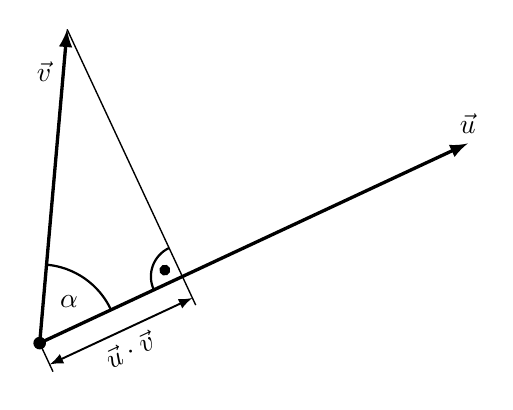
\begin{tikzpicture}[>=latex,thick]

\begin{scope}[rotate=25]

\def\a{60}
\def\l{4}
\def\r{1}

% Vektor u
\draw[->,line width=1.2pt] (0,0)--(6,0);
\node at (6,0) [above] {$\vec{u}$};

% Vektor v
\draw[->,line width=1.2pt] (0,0)--({\l*cos(\a)},{\l*sin(\a)});
\node at ({0.8*\l*cos(\a)},{0.8*\l*sin(\a)}) [above left] {$\vec{v}$};

% Projektion
\draw[line width=0.5pt] ({\l*cos(\a)},{\l*sin(\a)})--({\l*cos(\a)},-0.4);
\draw[line width=0.5pt] (0,0)--(0,-0.4);

% rechter Winkel
\def\rr{0.4}
\draw (2,\rr) arc (90:180:\rr);
\fill ({2-0.42*\rr},{0.42*\rr}) circle[radius=0.07];

% Winkel alpha
\draw (\r,0) arc (0:\a:\r);
\node at ({0.65*\r*cos(\a/2)},{0.65*\r*sin(\a/2)}) {$\alpha$};

% Bemassung
\draw[<->,line width=0.7pt] (0,-0.3)--({\l*cos(\a)},-0.3);
\node at ({0.5*\l*cos(\a)},-0.3) [below,rotate=25] {$\vec{u}\cdot\vec{v}$};

% Nullunkt
\fill (0,0) circle[radius=0.08];

\end{scope}

\end{tikzpicture}

\end{document}


%
% unendlich.tex -- Abschnitt über Dualraum unendlichdimensionaler Vektorräume
%
% (c) 2017 Prof Dr Andreas Müller, Hochschule Rapperswil
%
\section{Dualität und unendlichdimensionale Vektorräume%
\label{section:dualraum:unendlich}}
Für endlichdimensionale Vektorräume haben wir herausgefunden, dass
der Dualraum die gleiche Dimension hat, indem wir zu einer Basis die
duale Basis konstruiert haben.
Ein endlichdimensionaler Vektorraum und sein Dualraum haben daher die
gleiche Dimension.

Für unendlichdimensionale Vektorräume ist die Situation komplizierter.
Wir betrachten dazu einen Vektorraum $V$ mit einer Basis $B$, die jedoch
unendlich viele Elemente enthält.
Um die Situation nicht zu kompliziert werden zu lassen, nehmen wir an,
dass die Basis abzählbar ist, dass heisst dass die Basisvektoren 
numeriert werden können.
Wir schreiben sie
\[
B= \{ b_1,b_2,b_e,\dots\}.
\]
Natürlich können wir weiterhin die Linearformen $b_i^*$ konstruieren.
Das Lemma~\ref{dualraum:lemmaunabh} hat nicht vorausgesetzt, dass der
Vektorraum endlichdimensional muss, daher sind die dualen Linearformen
$b_i^*$ sicher linear unabhängig.

Trotzdem ist die Menge $B^*=\{b_i^*\;|\; i=\mathbb N\}$ keine Basis.
Wir können nämlich eine Linearform $l$ konstruieren, die sich nicht als 
Linearkombination der $b_i^*$ schreiben lässt.
Um den Wert von $l$ auf einem Vektor $v$ festzulegen, schreiben wir
zunächst
\[
v=v_0b_0+v_1b_1+v_2b_2+v_3b_3+\dots,
\]
wobei nur endlich viele der Koeffizienten $v_i$ von $0$ verschieden sind.
Als Wert von $l$ auf $v$ legen wir daher fest
\begin{equation}
l(v) = \sum_{i\in\mathbb N} v_i.
\label{dualraum:linf}
\end{equation}
Da nur endlich viele der $v_i$ von Null verschieden sind, ist die Summe
in \eqref{dualraum:linf} wohldefiniert.
In einem beliebigen Körper $K$ gibt es nämlich im Gegensatz zu den
Körpern $\mathbb R$ und $\mathbb C$ kein Konzept des Grenzwertes und
damit auch keine Möglichkeit, eine unendliche Summe zu berechnen.

Wir müssen jetzt noch einsehen, dass sich $l$ nicht als Linearkombination
von Linearformen $b_i^*$ geschreiben werden kann.
Wir zeigen dies dadurch, dass wir die Annahme, $l$ lasse sich als
Linearkombination der $b_i^*$ schreiben, zu einem Widerspruch führen.
Nehmen wir also an, dass 
\begin{equation}
l=l_0b_0^* + l_1b_1^*+l_2b_2^*+\dots+l_nb_n^*.
\label{dualraum:linf2}
\end{equation}
Wir haben eine endliche Summe geschrieben, weil in einem $K$-Vektorraum
unendliche Summen nicht definiert sind.
Eine Linearkombination kann daher immer nur endlich viele Summanden
enhalten.

Wir werten jetzt $l$ auf dem Basisvektor $b_{n+1}$ aus.
Aus der Definition wissen wir, dass $l(b_{n+1})=1$.
Setzen wir $b_{n+1}$ in die Darstellung 
\eqref{dualraum:linf2} von $l$ ein, erhalten wir
\[
1
=
l(b_{n+1})
=
l_0\underbrace{b_0^*(b_{n+1})}_{\displaystyle=0}
+
l_1\underbrace{b_1^*(b_{n+1})}_{\displaystyle=0}
+
l_2\underbrace{b_2^*(b_{n+1})}_{\displaystyle=0}
+\dots+
l_n\underbrace{b_n^*(b_{n+1})}_{\displaystyle=0}
=
0.
\]
Damit haben wir einen Widerspruch erhalten.
Es ist also nicht möglich, die Linearform $l$ als Linearkombination
von $b_i^*$ zu schreiben.

Dieses Beispiel zeigt, dass der Dualraum eines unendlichdimensionalen
Vektorraumes viele weitere Linearformen enthält, die sich nicht
als Linearkombinationen von $b_i^*$ schreiben lassen.
Man kann sogar zeigen, dass die es überabzählbar viele weitere, linear
unabhängige Linearformen gibt.
Ist nämlich $I\subset\mathbb N$ eine beliebige Teilmenge der natürlichen
Zahlen, dann können wir die Linearform $l_I$ definieren, die auf dem
Vektor $v$ den Wert
\[
l_I(v) = \sum_{i\in I}v_i
\]
haben soll.
Da nur endlich viele der Komponenten $v_i$ von $0$ verschieden sind, 
ist die Summe wohldefiniert.
Die oben beschriebene Linearform $l$ ist nichts anderers als $l_{\mathbb N}$.
Für jede unendliche Teilmenge $I$ ist $l_I$ eine Linearform, die nicht
durch die $b_i^*$ dargestellt werden kann.
Man kann sogar zeigen, dass es unter den $l_I$ überabzählbar viele 
linear unabhängige Linearformen gefunden werden können.
Eine Basis des Dualraumes $V^*$ ist daher viel grösser als eine Basis
von $V$.

Man kann diese Beobachtung auch als Indiz darauf betrachten, dass die
der Begriff des Vektorraumes für unendlichdimensionale Anwendungen noch
etwas zu wenig restriktiv ist.
Tatsächlich zeigt es sich, dass durch Hinzufügen eines Skalarproduktes
und von Grenzwerten eine sehr viel geeignetere Struktur entsteht,
der Hilbert-Raum.
Mehr dazu im Kapitel~\ref{chapter:hilbertspaces}.






